% ============================================================
% KHÓA LUẬN / DỰ ÁN TỐT NGHIỆP
% TRƯỜNG ĐẠI HỌC TÔN ĐỨC THẮNG – KHOA CÔNG NGHỆ THÔNG TIN
% Theo Quyết định số 884/2020/QĐ-TĐT, ngày 01/12/2020
% ============================================================

\documentclass[12pt, a4paper]{report}

\usepackage[utf8]{inputenc}
\usepackage[T5]{fontenc}
\usepackage[vietnamese, english]{babel}
\usepackage{csquotes}
\usepackage{mathptmx}

% Fix for texttt overflow: allow line breaks in \texttt
\usepackage[htt]{hyphenat}
\sloppy

\usepackage[
  a4paper,
  top    = 3.5cm,
  bottom = 3.0cm,
  left   = 3.5cm,
  right  = 2.0cm,
  headheight = 15pt,
]{geometry}

\usepackage{setspace}
\setstretch{1.5}

\usepackage{fancyhdr}
\pagestyle{fancy}
\fancyhf{}
\fancyhead[C]{\thepage}
\renewcommand{\headrulewidth}{0pt}
\fancypagestyle{plain}{
  \fancyhf{}
  \fancyhead[C]{\thepage}
  \renewcommand{\headrulewidth}{0pt}
}

\usepackage{indentfirst}
\setlength{\parindent}{1.27cm}

\usepackage{graphicx}
\usepackage{float}

\usepackage{caption}
\captionsetup{font=normalsize, labelsep=colon, justification=centering}

\usepackage{booktabs}
\usepackage{longtable}
\usepackage{multirow}
\usepackage{array}

\usepackage{amsmath}
\usepackage{amsfonts}
\usepackage{amssymb}

\usepackage[table]{xcolor}

\usepackage[
  colorlinks = true,
  linkcolor  = black,
  citecolor  = black,
  urlcolor   = blue,
]{hyperref}

\usepackage[
  style   = apa,
  backend = biber,
  sorting = nyt,
]{biblatex}
\addbibresource{references.bib}

\usepackage{acronym}
\usepackage{appendix}

\usepackage{titlesec}

% Chapter heading: "CHƯƠNG X.  TITLE" on a single line, bold, left-aligned
\titleformat{\chapter}[hang]
  {\normalfont\large\bfseries}
  {CHƯƠNG \thechapter.}
  {1em}
  {\large\bfseries\MakeUppercase}
\titlespacing*{\chapter}{0pt}{-20pt}{20pt}

% Starred chapters (LỜI CẢM ƠN, TÓM TẮT, etc.): centered, no prefix
\titleformat{name=\chapter,numberless}[block]
  {\normalfont\large\bfseries\centering}
  {}
  {0pt}
  {\large\bfseries}
\titlespacing*{name=\chapter,numberless}{0pt}{-20pt}{20pt}

\titleformat{\section}
  {\normalfont\normalsize\bfseries}{\thesection}{1em}{}
\titlespacing*{\section}{0pt}{12pt}{6pt}

\titleformat{\subsection}
  {\normalfont\normalsize\bfseries}{\thesubsection}{1em}{}
\titlespacing*{\subsection}{0pt}{10pt}{4pt}

\titleformat{\subsubsection}
  {\normalfont\normalsize\bfseries}{\thesubsubsection}{1em}{}
\titlespacing*{\subsubsection}{0pt}{8pt}{4pt}

\usepackage{chngcntr}
\counterwithin{figure}{chapter}
\counterwithin{table}{chapter}
\counterwithin{equation}{chapter}
\renewcommand{\theequation}{\thechapter.\arabic{equation}}

\addto\captionsenglish{%
  \renewcommand{\figurename}{Hình}%
  \renewcommand{\tablename}{Bảng}%
  \renewcommand{\contentsname}{MỤC LỤC}%
  \renewcommand{\listfigurename}{DANH MỤC HÌNH VẼ}%
  \renewcommand{\listtablename}{DANH MỤC BẢNG BIỂU}%
  \renewcommand{\bibname}{TÀI LIỆU THAM KHẢO}%
  \renewcommand{\chaptername}{CHƯƠNG}%
  \renewcommand{\appendixname}{PHỤ LỤC}%
}

\newcommand{\thesistitle}{HỆ THỐNG CHẤM BÀI TRỰC TUYẾN - TDTUOJ}
\newcommand{\thesistitleen}{ONLINE JUDGE SYSTEM - TDTUOJ}
\newcommand{\studentone}{Hồ Nguyễn An Khang -- 52200020}
\newcommand{\supervisor}{ThS. Doãn Xuân Thanh}
\newcommand{\major}{Kỹ thuật phần mềm}
\newcommand{\submityear}{2026}

% ============================================================
\begin{document}
% ============================================================

\fontsize{13pt}{15.6pt}\selectfont
\pagenumbering{gobble}

% ------------------------------------------------------------
% TRANG BÌA CHÍNH (Mẫu 1)
% ------------------------------------------------------------
\begin{titlepage}
  \begin{center}
    \textbf{TỔNG LIÊN ĐOÀN LAO ĐỘNG VIỆT NAM}\\[0.3cm]
    \textbf{TRƯỜNG ĐẠI HỌC TÔN ĐỨC THẮNG}\\[0.3cm]
    \textbf{KHOA CÔNG NGHỆ THÔNG TIN}\\[1cm]
    
\includegraphics[width=0.25\textwidth]{figures/logo.png}\\[1cm]
    {\large\textbf{\studentone}}\\[2.5cm]
    {\Large\textbf{\MakeUppercase{\thesistitle}}}\\[1.5cm]
    {\large\textbf{KHÓA LUẬN TỐT NGHIỆP}}\\[0.5cm]
    {\normalsize\textbf{\major}}\\[0.5cm]
    \vfill
    \textbf{THÀNH PHỐ HỒ CHÍ MINH, NĂM \submityear}
  \end{center}
\end{titlepage}

% ------------------------------------------------------------
% TRANG BÌA PHỤ (Mẫu 2)
% ------------------------------------------------------------
\begin{titlepage}
  \begin{center}
    \textbf{TỔNG LIÊN ĐOÀN LAO ĐỘNG VIỆT NAM}\\[0.3cm]
    \textbf{TRƯỜNG ĐẠI HỌC TÔN ĐỨC THẮNG}\\[0.3cm]
    \textbf{KHOA CÔNG NGHỆ THÔNG TIN}\\[1cm]
    
\includegraphics[width=0.25\textwidth]{figures/logo.png}\\[1cm]
    {\large\textbf{\studentone}}\\[2.5cm]
    {\Large\textbf{\MakeUppercase{\thesistitle}}}\\[1.5cm]
    {\large\textbf{KHÓA LUẬN TỐT NGHIỆP}}\\[0.5cm]
    {\normalsize\textbf{\major}}\\[1.5cm]
    Người hướng dẫn:\\[0.2cm]
    \textbf{\supervisor}
    \vfill
    \textbf{THÀNH PHỐ HỒ CHÍ MINH, NĂM \submityear}
  \end{center}
\end{titlepage}

% ------------------------------------------------------------
% LỜI CẢM ƠN
% ------------------------------------------------------------
\chapter*{LỜI CẢM ƠN}
\addcontentsline{toc}{chapter}{LỜI CẢM ƠN}

Em xin chân thành cảm ơn quý thầy cô Khoa Công nghệ Thông tin, Trường Đại học Tôn Đức Thắng đã tận tình giảng dạy và trang bị cho em những kiến thức nền tảng vững chắc trong suốt quá trình học tập. Đặc biệt, em xin gửi lời cảm ơn sâu sắc đến giảng viên hướng dẫn \textbf{\supervisor} đã dành thời gian định hướng, góp ý và hỗ trợ em trong từng giai đoạn thực hiện đề tài này. Bên cạnh đó, em xin cảm ơn gia đình và bạn bè đã luôn động viên, tạo điều kiện để em có thể hoàn thành tốt dự án.

\vspace{3cm}
\begin{flushright}
  \begin{minipage}{10cm}
    \centering
    TP. Hồ Chí Minh, ngày \ldots{} tháng \ldots{} năm 20\ldots{}\\[1cm]
    \textbf{Tác giả}\\[0.3cm]
    (\textit{Ký tên và ghi rõ họ tên})
  \end{minipage}
\end{flushright}
\newpage

% ------------------------------------------------------------
% LỜI CAM ĐOAN
% ------------------------------------------------------------
\chapter*{LỜI CAM ĐOAN}
\addcontentsline{toc}{chapter}{LỜI CAM ĐOAN}

\begin{center}
  \textbf{CÔNG TRÌNH ĐƯỢC HOÀN THÀNH\\
  TẠI TRƯỜNG ĐẠI HỌC TÔN ĐỨC THẮNG}
\end{center}

\noindent Tôi xin cam đoan đây là công trình nghiên cứu của riêng tôi và được sự hướng dẫn khoa học của \textbf{\supervisor}. Các nội dung nghiên cứu, kết quả trong đề tài này là trung thực và chưa công bố dưới bất kỳ hình thức nào trước đây. Những số liệu trong các bảng biểu phục vụ cho việc phân tích, nhận xét, đánh giá được chính tác giả thu thập từ các nguồn khác nhau có ghi rõ trong phần tài liệu tham khảo.

\noindent Ngoài ra, trong Dự án còn sử dụng một số nhận xét, đánh giá cũng như số liệu của các tác giả khác, cơ quan tổ chức khác đều có trích dẫn và chú thích nguồn gốc.

\noindent Nếu phát hiện có bất kỳ sự gian lận nào tôi xin hoàn toàn chịu trách nhiệm về nội dung Dự án của mình. Trường Đại học Tôn Đức Thắng không liên quan đến những vi phạm tác quyền, bản quyền do tôi gây ra trong quá trình thực hiện (nếu có).

\vspace{3cm}
\begin{flushright}
  \begin{minipage}{10cm}
    \centering
    TP. Hồ Chí Minh, ngày \ldots{} tháng \ldots{} năm 20\ldots{}\\[1cm]
    \textbf{Tác giả}\\[0.3cm]
    (\textit{Ký tên và ghi rõ họ tên})
  \end{minipage}
\end{flushright}
\newpage

% ------------------------------------------------------------
% TÓM TẮT
% ------------------------------------------------------------
\chapter*{\thesistitle}
\addcontentsline{toc}{chapter}{TÓM TẮT}
\begin{center}\textbf{TÓM TẮT}\end{center}

\noindent Dự án này trình bày quá trình nghiên cứu, thiết kế và triển khai ban đầu của Hệ thống Chấm bài Trực tuyến TDTUOJ -- một nền tảng được xây dựng nhằm tự động hóa quy trình chấm bài lập trình và hỗ trợ tổ chức thi cử cho sinh viên Khoa Công nghệ Thông tin, Trường Đại học Tôn Đức Thắng.

\noindent Hệ thống được thiết kế để phục vụ ba nhóm người dùng chính gồm sinh viên, giảng viên và quản trị viên, với các chức năng cốt lõi bao gồm nộp và chấm bài tự động cho nhiều ngôn ngữ lập trình, quản lý cuộc thi và bài toán, và phân tích hỗ trợ học tập thông minh bằng \ac{LLM}. Kiến trúc hệ thống được xây dựng theo mô hình hai lớp tách biệt rõ ràng giữa backend và frontend, tích hợp với ba dịch vụ bên ngoài gồm Judging Service (Judge0), \ac{LLM} và AI Parser Service.

\noindent Đến thời điểm báo cáo giữa kỳ, hệ thống đã hoàn thành phần lớn các chức năng cốt lõi. Phía backend được xây dựng bằng Java với Spring Boot, đã hiện thực hóa đầy đủ các \ac{API} quản lý người dùng, quản lý bài toán và luồng xử lý bài nộp tích hợp Judge0. Phía frontend được xây dựng bằng React, đã hoàn thiện giao diện xem chi tiết bài toán theo slug, quản lý người dùng, tính năng nộp bài và hỗ trợ học tập bằng \ac{LLM}.

\newpage

\chapter*{\thesistitleen}
\addcontentsline{toc}{chapter}{ABSTRACT}
\begin{center}\textbf{ABSTRACT}\end{center}

\noindent This project presents the research, design, and initial implementation of the TDTUOJ Online Judge System -- a platform built to automate programming submission grading and support examination organization for students of the Faculty of Information Technology at Ton Duc Thang University.

\noindent The system is designed to serve three main user groups: students, lecturers, and administrators, with core features including automatic submission judging for multiple programming languages via Judge0, contest and problem management, and AI-powered learning support via \ac{LLM} integration. The system architecture follows a clear two-layer separation between a Java Spring Boot backend and a React frontend, integrated with three external services: Judging Service (Judge0), \ac{LLM}, and AI Parser Service.

\noindent As of the midterm report, the majority of core features have been implemented. The backend provides complete \ac{API} coverage for user management, problem management, and Judge0-integrated submission processing. The frontend has completed the problem detail view by slug, user management interface, submission functionality, and \ac{LLM}-powered hint and code explanation features.

\newpage

% ── Roman page numbers ───────────────────────────────────────
\pagenumbering{roman}
\setcounter{page}{1}

\tableofcontents
\newpage

\listoffigures
\addcontentsline{toc}{chapter}{DANH MỤC HÌNH VẼ}
\newpage

\listoftables
\addcontentsline{toc}{chapter}{DANH MỤC BẢNG BIỂU}
\newpage

% ------------------------------------------------------------
% DANH MỤC CÁC CHỮ VIẾT TẮT
% ------------------------------------------------------------
\chapter*{DANH MỤC CÁC CHỮ VIẾT TẮT}
\addcontentsline{toc}{chapter}{DANH MỤC CÁC CHỮ VIẾT TẮT}

\begin{acronym}[XXXXXXXX]
  \acro{AC}{Accepted}
  \acro{AI}{Artificial Intelligence -- Trí tuệ nhân tạo}
  \acro{API}{Application Programming Interface}
  \acro{CE}{Compilation Error}
  \acro{CNTT}{Công nghệ Thông tin}
  \acro{CSS}{Cascading Style Sheets}
  \acro{ERD}{Entity-Relationship Diagram -- Sơ đồ thực thể quan hệ}
  \acro{HTTP}{Hypertext Transfer Protocol}
  \acro{JPA}{Java Persistence API}
  \acro{JSON}{JavaScript Object Notation}
  \acro{JWT}{JSON Web Token}
  \acro{LLM}{Large Language Model -- Mô hình ngôn ngữ lớn}
  \acro{MLE}{Memory Limit Exceeded}
  \acro{MVC}{Model-View-Controller}
  \acro{OJ}{Online Judge}
  \acro{PDF}{Portable Document Format}
  \acro{PK}{Primary Key -- Khóa chính}
  \acro{FK}{Foreign Key -- Khóa ngoại}
  \acro{RE}{Runtime Error}
  \acro{REST}{Representational State Transfer}
  \acro{TDTU}{Trường Đại học Tôn Đức Thắng}
  \acro{TLE}{Time Limit Exceeded}
  \acro{UI}{User Interface}
  \acro{UX}{User Experience}
  \acro{WA}{Wrong Answer}
\end{acronym}
\newpage

% ── Arabic page numbers from 1 ───────────────────────────────
\pagenumbering{arabic}
\setcounter{page}{1}

% ============================================================
% CHƯƠNG 1 – MỞ ĐẦU VÀ TỔNG QUAN ĐỀ TÀI
% ============================================================
\chapter{Mở đầu và tổng quan đề tài}

\section{Đặt vấn đề}

Hiện nay, việc tổ chức các kỳ thi lập trình và rèn luyện kỹ năng giải thuật cho sinh viên tại Trường Đại học Tôn Đức Thắng vẫn còn nhiều hạn chế về mặt công cụ hỗ trợ. Chấm bài thủ công tiêu tốn nhiều thời gian và công sức của giảng viên, đồng thời khó đảm bảo tính nhất quán khi số lượng sinh viên ngày càng tăng. Bên cạnh đó, sinh viên thiếu một môi trường luyện tập chủ động với phản hồi tức thì để tự nâng cao kỹ năng lập trình ngoài giờ học.

Để giải quyết những vấn đề này, đề tài đề xuất xây dựng Hệ thống Chấm bài Trực tuyến TDTUOJ -- một nền tảng tự động hóa toàn bộ quy trình chấm bài, hỗ trợ tổ chức thi cử quy mô lớn và tạo ra môi trường luyện tập lập trình chuyên nghiệp trong khuôn khổ học thuật của nhà trường.

\section{Mục tiêu của hệ thống}

TDTUOJ được xây dựng nhằm đạt một tập hợp các mục tiêu cụ thể và có tính ứng dụng cao. Về mặt kỹ thuật, hệ thống hỗ trợ đa ngôn ngữ lập trình, cho phép người dùng nộp bài viết bằng C, C++, Java và Python, đáp ứng nhu cầu đa dạng của sinh viên ở nhiều trình độ và môn học khác nhau. Song song với đó, hệ thống cung cấp đầy đủ công cụ để quản lý cuộc thi và bài tập, bao gồm tổ chức contest, quản lý danh sách bài toán, chấm điểm tự động và xếp hạng người tham gia theo thời gian thực.

Ngoài các chức năng cốt lõi, hệ thống tích hợp một số tính năng nâng cao phục vụ học tập. Tính năng phân tích mã nguồn bằng \ac{LLM} cho phép giải thích code, gợi ý hướng giải và phân tích độ phức tạp thuật toán ngay trên giao diện -- giúp sinh viên hiểu rõ hơn về hiệu suất và logic của giải pháp mình đề xuất. Ngoài ra, hệ thống tích hợp AI Parser Service để tự động đọc đề bài từ file \ac{PDF} và chuyển đổi thành dữ liệu có cấu trúc, giúp giảng viên tiết kiệm đáng kể thời gian soạn thảo.

\section{Phạm vi đề tài}

Đề tài tập trung xây dựng một hệ thống hoàn chỉnh phục vụ sinh viên và giảng viên Khoa Công nghệ Thông tin, Trường Đại học Tôn Đức Thắng. Hệ thống quản lý ba vai trò với phân quyền rõ ràng: User (người dùng thông thường), Contest Creator (người tổ chức và quản lý cuộc thi), và Admin (quản trị viên với toàn quyền điều hành). Về mặt kiến trúc, phạm vi đề tài bao gồm phát triển một backend \ac{REST}ful \ac{API} bằng Java Spring Boot, một giao diện người dùng bằng React, và tích hợp ba dịch vụ bên ngoài: Judging Service (Judge0), \ac{LLM} và AI Parser Service.

% ============================================================
% CHƯƠNG 2 – CÔNG NGHỆ SỬ DỤNG
% ============================================================
\chapter{Công nghệ sử dụng}

Hệ thống TDTUOJ được xây dựng trên nền tảng các công nghệ hiện đại, được lựa chọn có chủ đích để đảm bảo hiệu năng, khả năng mở rộng và dễ dàng bảo trì. Chương này trình bày chi tiết từng công nghệ được áp dụng, lý do lựa chọn và cách thức tích hợp vào hệ thống.

\section{Backend -- Java và Spring Boot}

\subsection{Tổng quan về Spring Boot}

Spring Boot là một framework mã nguồn mở được phát triển bởi Pivotal (nay là VMware), xây dựng trên nền tảng Spring Framework của Java. Spring Boot ra đời nhằm giải quyết một trong những điểm yếu lịch sử của Spring Framework truyền thống -- đó là sự phức tạp trong cấu hình. Thay vì yêu cầu lập trình viên tự cấu hình hàng trăm dòng XML hoặc annotation, Spring Boot áp dụng triết lý \textit{convention over configuration} (ưu tiên quy ước hơn cấu hình), tự động phát hiện và cấu hình các thành phần dựa trên các thư viện có mặt trong classpath.

Cơ chế trung tâm của Spring Boot là \textit{Auto-configuration} -- khi thêm dependency \texttt{spring-boot-starter-web} vào dự án, Spring Boot tự động khởi tạo một máy chủ Tomcat nhúng, cấu hình DispatcherServlet và thiết lập Jackson để xử lý JSON mà không cần bất kỳ cấu hình thủ công nào. Điều này giúp lập trình viên tập trung vào logic nghiệp vụ thay vì quản lý cơ sở hạ tầng.

Spring Boot cũng cung cấp hệ sinh thái \textit{Starter dependencies} phong phú, mỗi starter đóng gói một tập hợp các thư viện liên quan: \texttt{spring-boot-starter-data-jpa} tích hợp Hibernate và Spring Data JPA, \texttt{spring-boot-starter-security} cung cấp toàn bộ khung bảo mật, và \texttt{spring-boot-starter-test} tích hợp JUnit, Mockito và các công cụ kiểm thử khác.

\subsection{Kiến trúc MVC trong TDTUOJ}

TDTUOJ áp dụng kiến trúc \ac{MVC} kết hợp với mô hình \ac{REST}ful \ac{API}. Trong Spring Boot, kiến trúc này được tổ chức thành các lớp tách biệt rõ ràng:

Lớp \textbf{Controller} đảm nhận vai trò tiếp nhận các \ac{HTTP} request từ frontend. Mỗi controller được đánh dấu bằng annotation \texttt{@RestController} và định nghĩa các endpoint thông qua \texttt{@GetMapping}, \texttt{@PostMapping}, \texttt{@PutMapping} và \texttt{@DeleteMapping}. Ví dụ, \texttt{ProblemController} xử lý toàn bộ các request liên quan đến bài toán, từ lấy danh sách, xem chi tiết theo slug đến tạo mới và cập nhật.

Lớp \textbf{Service} chứa toàn bộ logic nghiệp vụ, được đánh dấu bằng \texttt{@Service}. Đây là nơi thực thi các quy tắc kinh doanh như kiểm tra quyền hạn người dùng, xử lý trạng thái bài nộp, tính điểm cuộc thi và gọi các dịch vụ bên ngoài.

Lớp \textbf{Repository} tương tác trực tiếp với cơ sở dữ liệu thông qua Spring Data \ac{JPA}. Các interface kế thừa \texttt{JpaRepository} được Spring Boot tự động hiện thực, cung cấp sẵn các phương thức CRUD mà không cần viết câu lệnh SQL thủ công. Truy vấn tùy chỉnh có thể được định nghĩa bằng cú pháp \texttt{findBy...} hoặc annotation \texttt{@Query} với ngôn ngữ JPQL.

\subsection{Bảo mật với Spring Security và JWT}

Hệ thống TDTUOJ sử dụng \ac{JWT} để xác thực và phân quyền người dùng. Cơ chế hoạt động như sau: sau khi đăng nhập thành công, backend tạo ra một JWT chứa thông tin định danh người dùng và vai trò của họ, ký bằng khóa bí mật và trả về cho client. Với mỗi request tiếp theo, client đính kèm token trong header \texttt{Authorization: Bearer <token>}, backend kiểm tra tính hợp lệ của token trước khi xử lý request.

Spring Security được cấu hình với một \texttt{JwtAuthenticationFilter} tùy chỉnh, chặn mọi request đến và xác minh token trước khi cho phép đi qua. Phân quyền được thực thi tại lớp controller thông qua annotation \texttt{@PreAuthorize}, cho phép kiểm soát chi tiết đến từng endpoint -- chẳng hạn chỉ Admin mới có thể gọi các API quản lý tài khoản, trong khi Contest Creator mới có thể tạo cuộc thi.

\section{Cơ sở dữ liệu -- PostgreSQL}

\subsection{Tổng quan về PostgreSQL}

PostgreSQL là hệ quản trị cơ sở dữ liệu quan hệ mã nguồn mở mạnh mẽ, nổi tiếng với khả năng tuân thủ chuẩn SQL nghiêm ngặt, hỗ trợ các kiểu dữ liệu phong phú và độ ổn định cao trong môi trường production. So với MySQL, PostgreSQL có ưu thế trong việc xử lý các truy vấn phức tạp với nhiều phép JOIN, hỗ trợ các kiểu dữ liệu đặc biệt như \texttt{JSONB}, \texttt{ARRAY} và \texttt{UUID}, và có cơ chế kiểm soát đồng thời đa phiên bản (MVCC) hiệu quả hơn trong các tình huống ghi/đọc đồng thời -- rất phù hợp với kịch bản nhiều người dùng cùng nộp bài trong một cuộc thi.

Trong TDTUOJ, PostgreSQL được chọn làm cơ sở dữ liệu chính, lưu trữ toàn bộ 20 bảng mô tả trong sơ đồ \ac{ERD}. Spring Data \ac{JPA} với Hibernate làm ORM layer đảm nhận việc ánh xạ giữa các entity Java và các bảng trong cơ sở dữ liệu.

\subsection{Cấu hình kết nối}

Kết nối từ Spring Boot đến PostgreSQL được cấu hình trong file \texttt{application.pro\-perties} với các thông số \texttt{spring.data\-source.url}, \texttt{spring.data\-source.user\-name} và \texttt{spring.data\-source.pass\-word}. Connection pooling được quản lý bởi HikariCP -- pool kết nối mặc định và hiệu năng cao nhất của Spring Boot -- giúp tái sử dụng kết nối và giảm độ trễ khi có nhiều request đồng thời.

\section{Docker và Containerization}

\subsection{Tổng quan về Docker}

Docker là nền tảng container hóa cho phép đóng gói ứng dụng cùng toàn bộ môi trường phụ thuộc (runtime, thư viện, biến môi trường, file cấu hình) vào một đơn vị gọi là \textit{container}. Khác với máy ảo truyền thống phải ảo hóa toàn bộ hệ điều hành, container chia sẻ kernel của máy chủ, giúp khởi động nhanh hơn, tiêu tốn ít tài nguyên hơn và dễ dàng di chuyển giữa các môi trường.

\subsection{Containerization Judge0 với Docker}

Judge0 là dịch vụ chấm bài mã nguồn mở được triển khai thông qua Docker. Hệ thống Judge0 bao gồm nhiều thành phần phối hợp với nhau, được quản lý bằng Docker Compose:

\begin{itemize}
  \item \textbf{judge0-server}: Container chính cung cấp \ac{REST}ful \ac{API} để nhận bài nộp và trả về kết quả.
  \item \textbf{judge0-workers}: Các worker container thực thi mã nguồn trong môi trường sandbox cô lập, sử dụng \textit{isolate} -- một công cụ kiểm soát tài nguyên dựa trên Linux cgroups và namespaces.
  \item \textbf{Redis}: Hàng đợi bài nộp, lưu trữ các submission đang chờ được xử lý bởi worker.
  \item \textbf{PostgreSQL}: Cơ sở dữ liệu nội bộ của Judge0, lưu kết quả và lịch sử chấm bài.
\end{itemize}

Cấu hình triển khai Judge0 bằng Docker Compose được mô tả như sau:

\begin{verbatim}
services:
  server:
    image: judge0/judge0:latest
    ports:
      - "2358:2358"
    environment:
      REDIS_HOST: redis
      POSTGRES_HOST: db
    depends_on:
      - redis
      - db

  workers:
    image: judge0/judge0:latest
    command: ["./scripts/workers"]
    privileged: true
    depends_on:
      - server

  redis:
    image: redis:7-alpine

  db:
    image: postgres:16-alpine
    environment:
      POSTGRES_PASSWORD: judge0
\end{verbatim}

Lưu ý quan trọng: container \texttt{workers} cần được chạy với quyền \texttt{privileged: true} vì \textit{isolate} cần quyền truy cập kernel-level để tạo ra các cgroups và namespaces kiểm soát tài nguyên. Backend TDTUOJ giao tiếp với Judge0 thông qua \ac{API} tại cổng \texttt{2358}, gửi mã nguồn kèm theo ngôn ngữ lập trình và giới hạn thời gian/bộ nhớ lấy từ bảng \texttt{test\_cases}.

\subsection{Docker Compose cho toàn hệ thống}

Ngoài Judge0, toàn bộ môi trường phát triển của TDTUOJ cũng được container hóa. File \texttt{docker-compose.yml} của dự án tổ chức các dịch vụ sau:

\begin{itemize}
  \item \textbf{tdtuoj-backend}: Container chạy Spring Boot application, được build từ \texttt{Dockerfile} trong thư mục \texttt{TDTUOJ\_backend}.
  \item \textbf{tdtuoj-postgres}: Container PostgreSQL phục vụ dữ liệu của TDTUOJ, độc lập với PostgreSQL của Judge0.
  \item \textbf{tdtuoj-frontend}: Container React application phục vụ giao diện người dùng.
\end{itemize}

Việc sử dụng Docker giúp đảm bảo tính nhất quán giữa môi trường phát triển của từng thành viên và môi trường production, đồng thời đơn giản hóa quá trình thiết lập -- thay vì cài đặt Java, Node.js, PostgreSQL riêng lẻ, người phát triển chỉ cần chạy \texttt{docker-compose up} để khởi động toàn bộ hệ thống.

\section{Redis -- Hàng đợi và Bộ nhớ đệm}

\subsection{Tổng quan về Redis}

Redis (Remote Dictionary Server) là một kho lưu trữ dữ liệu trong bộ nhớ (in-memory data store) mã nguồn mở, thường được sử dụng như một cơ sở dữ liệu tốc độ cao, bộ nhớ đệm (cache) và message broker. Điểm khác biệt cơ bản của Redis so với các hệ quản trị cơ sở dữ liệu truyền thống là toàn bộ dữ liệu được lưu trong RAM thay vì đĩa cứng, cho phép đạt tốc độ đọc/ghi cực cao -- thường đạt hàng trăm nghìn thao tác mỗi giây. Redis hỗ trợ nhiều cấu trúc dữ liệu phong phú như string, hash, list, set, sorted set và stream, mỗi loại phù hợp với một bài toán cụ thể.

Trong TDTUOJ, Redis được sử dụng theo hai mục đích chính: làm hàng đợi bài nộp (submission queue) để xử lý bất đồng bộ với Judge0, và làm bộ nhớ đệm cho bảng xếp hạng (leaderboard cache) trong các cuộc thi.

\subsection{Hàng đợi bài nộp với Redis}

Khi nhiều người dùng nộp bài cùng lúc -- đặc biệt trong các cuộc thi có hàng trăm thí sinh -- hệ thống phải xử lý một lượng lớn submission đồng thời. Nếu backend gửi trực tiếp từng submission đến Judge0 và chờ kết quả ngay lập tức (synchronous), các request sẽ chiếm giữ thread trong suốt thời gian Judge0 thực thi mã nguồn, dẫn đến hiện tượng thread pool cạn kiệt và hệ thống trở nên không phản hồi.

Để giải quyết vấn đề này, TDTUOJ áp dụng mô hình hàng đợi bất đồng bộ với Redis theo luồng sau:

Khi người dùng nộp bài, backend không gọi Judge0 trực tiếp mà thay vào đó tạo một bản ghi \texttt{submission} với trạng thái \texttt{PENDING} trong cơ sở dữ liệu, sau đó đẩy một message chứa \texttt{submission\_id} vào một Redis List (đóng vai trò hàng đợi) và lập tức trả về phản hồi cho người dùng. Người dùng nhận được xác nhận bài đã được tiếp nhận mà không phải chờ kết quả chấm.

Ở phía tiêu thụ hàng đợi, một hoặc nhiều \textit{submission worker} chạy nền liên tục lắng nghe hàng đợi Redis bằng lệnh \texttt{BLPOP} (blocking left pop) -- lệnh này chặn worker cho đến khi có message mới xuất hiện trong hàng đợi, tránh việc polling liên tục tiêu tốn CPU. Khi nhận được \texttt{submission\_id}, worker truy xuất thông tin submission và test cases từ cơ sở dữ liệu, gửi lần lượt từng test case đến Judge0 \ac{API}, nhận về kết quả, tổng hợp verdict cuối cùng và cập nhật bản ghi trong bảng \texttt{submissions} từ trạng thái \texttt{PENDING} sang \texttt{JUDGED}.

Luồng này có thể được mô tả qua các bước tuần tự sau:

\begin{enumerate}
  \item Frontend gửi \texttt{POST /submissions} đến backend.
  \item Backend lưu submission với trạng thái \texttt{PENDING}, đẩy \texttt{submission\_id} vào Redis List \texttt{submission\_queue}.
  \item Backend trả về \texttt{HTTP 202 Accepted} cùng \texttt{submission\_id} cho frontend.
  \item Frontend polling endpoint \texttt{GET /submissions/\{id\}} theo chu kỳ để kiểm tra trạng thái.
  \item Worker nhận \texttt{submission\_id} từ hàng đợi, gửi đến Judge0, nhận verdict và cập nhật cơ sở dữ liệu.
  \item Lần polling tiếp theo của frontend nhận được kết quả đã hoàn chỉnh.
\end{enumerate}

Mô hình này mang lại hai lợi ích quan trọng: thứ nhất, hệ thống có khả năng mở rộng theo chiều ngang bằng cách tăng số lượng worker xử lý song song khi tải cao; thứ hai, các submission không bao giờ bị mất -- nếu một worker gặp sự cố trong khi xử lý, message vẫn có thể được xử lý lại thay vì bị bỏ qua hoàn toàn.

\subsection{Bộ nhớ đệm bảng xếp hạng}

Trong thời gian diễn ra cuộc thi, bảng xếp hạng cần được cập nhật liên tục và phục vụ hàng trăm request xem leaderboard đồng thời. Nếu mỗi request đều thực hiện truy vấn tổng hợp phức tạp trên bảng \texttt{contest\_participations} -- tính điểm, sắp xếp, phân trang -- thì cơ sở dữ liệu sẽ chịu tải rất lớn và thời gian phản hồi sẽ tăng cao.

TDTUOJ giải quyết vấn đề này bằng cách sử dụng Redis làm lớp cache cho bảng xếp hạng, phản ánh thiết kế của bảng \texttt{leaderboard\_cache} trong sơ đồ \ac{ERD}. Sau mỗi lần có bài nộp được chấp nhận trong cuộc thi, hệ thống tính toán lại thứ hạng và lưu kết quả đã được serialize vào Redis với một TTL (time-to-live) ngắn. Các request xem bảng xếp hạng tiếp theo đọc trực tiếp từ Redis thay vì truy vấn cơ sở dữ liệu, giúp thời gian phản hồi giảm từ hàng trăm millisecond xuống còn dưới một millisecond. Khi TTL hết hạn hoặc có cập nhật mới, cache được làm mới tự động, đảm bảo tính nhất quán giữa dữ liệu hiển thị và trạng thái thực tế của cuộc thi.

\section{Judging Service -- Judge0}

\subsection{Tổng quan về Judge0}

Judge0 là một dịch vụ chấm bài mã nguồn mở, cung cấp môi trường thực thi mã nguồn an toàn và cô lập hỗ trợ hơn 60 ngôn ngữ lập trình. Thay vì tự xây dựng cơ sở hạ tầng sandbox từ đầu -- một bài toán kỹ thuật phức tạp đòi hỏi kiến thức sâu về bảo mật hệ điều hành -- TDTUOJ tích hợp Judge0 như một dịch vụ độc lập có thể gọi qua \ac{API}.

\subsection{Luồng xử lý bài nộp}

Luồng tích hợp Judge0 trong TDTUOJ được thực thi theo các bước sau. Đầu tiên, khi người dùng nhấn nộp bài trên frontend, một \ac{HTTP} POST request được gửi đến backend kèm theo mã nguồn, ngôn ngữ lập trình và thông tin bài toán. Backend đọc danh sách test cases từ bảng \texttt{test\_cases} và gửi từng test case đến endpoint \texttt{POST /submissions} của Judge0, kèm theo \texttt{source\_code}, \texttt{language\_id}, \texttt{stdin} (đầu vào), \texttt{expected\_output}, \texttt{cpu\_time\_limit} và \texttt{memory\_limit}.

Judge0 nhận request, đưa vào hàng đợi Redis và phân công cho một worker xử lý. Worker thực thi mã nguồn trong môi trường sandbox cô lập, so sánh đầu ra với \texttt{expected\_output} và trả về token định danh. Backend poll kết quả theo token đó, nhận về verdict tương ứng: \ac{AC}, \ac{WA}, \ac{TLE}, \ac{MLE}, \ac{RE} hoặc \ac{CE}. Sau khi nhận đủ kết quả của tất cả test cases, backend tổng hợp verdict cuối cùng và lưu vào bảng \texttt{submissions}.

Toàn bộ luồng này được thiết kế bất đồng bộ ở phía backend: thread xử lý request không bị chặn trong khi chờ Judge0 -- backend sử dụng cơ chế polling hoặc webhook để nhận kết quả, đảm bảo khả năng xử lý nhiều bài nộp song song mà không làm ảnh hưởng đến hiệu năng tổng thể.

\section{Frontend -- React}

\subsection{Tổng quan về React}

React là thư viện JavaScript mã nguồn mở được Meta phát triển, chuyên dùng để xây dựng giao diện người dùng. Điểm cốt lõi của React là mô hình lập trình khai báo (declarative) dựa trên \textit{component} -- mỗi phần của giao diện được đóng gói thành một component độc lập với state và logic riêng, có thể tái sử dụng ở nhiều nơi trong ứng dụng.

React sử dụng \textit{Virtual DOM} -- một bản sao nhẹ của DOM thực trong bộ nhớ. Khi state thay đổi, React tính toán sự khác biệt (diffing) giữa Virtual DOM cũ và mới, sau đó chỉ cập nhật đúng những phần thực sự thay đổi trên DOM thực. Cơ chế này giúp tối ưu hiệu năng đáng kể so với việc thao tác DOM trực tiếp.

\subsection{Cấu trúc ứng dụng React trong TDTUOJ}

Frontend của TDTUOJ được xây dựng theo mô hình SPA (\textit{Single Page Application}) sử dụng React Router để điều hướng giữa các trang mà không cần tải lại toàn bộ trang. Cấu trúc thư mục được tổ chức theo tính năng: mỗi module lớn như quản lý bài toán, cuộc thi, người dùng và nộp bài được đặt trong thư mục riêng, chứa các component, hook tùy chỉnh và file gọi \ac{API} tương ứng.

Giao tiếp với backend thực hiện qua \ac{HTTP} request sử dụng Fetch API, với \ac{JWT} được đính kèm trong header \texttt{Authorization} của mỗi request yêu cầu xác thực. Dữ liệu trao đổi theo định dạng \ac{JSON}, được React tự động cập nhật vào state component thông qua các hook \texttt{useState} và \texttt{useEffect}.

\section{Lưu trữ file -- AWS S3}

Nội dung đề bài và dữ liệu test cases được lưu trữ trên \textbf{AWS} S3 (Simple Storage Service) -- dịch vụ lưu trữ đối tượng có khả năng mở rộng không giới hạn của Amazon. Thay vì lưu trực tiếp trong cơ sở dữ liệu, các file lớn như đề bài định dạng \ac{PDF} và file input/output của test cases được upload lên S3 bucket, còn cơ sở dữ liệu chỉ lưu đường dẫn URL trỏ đến các file đó -- thể hiện qua các trường \texttt{statement\_file\_url}, \texttt{input\_file\_url} và \texttt{expected\_output\_file\_url} trong thiết kế bảng. Cách tiếp cận này giúp cơ sở dữ liệu không bị phình to, đồng thời tận dụng được khả năng phân phối nội dung toàn cầu và độ bền lưu trữ cao của S3.

\section{Tích hợp LLM}

Hệ thống tích hợp \ac{LLM} thông qua \ac{API} để cung cấp ba tính năng hỗ trợ học tập: phân tích độ phức tạp thuật toán, giải thích mã nguồn và lỗi, và gợi ý hướng giải quyết bài toán. Backend đóng vai trò trung gian -- tiếp nhận yêu cầu từ frontend, xây dựng prompt phù hợp chứa ngữ cảnh bài toán và mã nguồn của người dùng, gửi đến \ac{LLM} \ac{API} và trả kết quả về frontend để hiển thị. Kiến trúc này tách biệt hoàn toàn việc gọi \ac{LLM} khỏi frontend, giúp bảo vệ API key và cho phép thay đổi nhà cung cấp \ac{LLM} mà không ảnh hưởng đến giao diện.

% ============================================================
% CHƯƠNG 3 – PHÂN TÍCH HỆ THỐNG
% ============================================================
\chapter{Phân tích hệ thống}

\section{Kiến trúc tổng quan}

TDTUOJ được xây dựng theo kiến trúc tách biệt hoàn toàn giữa backend và frontend, trong đó backend đóng vai trò máy chủ cung cấp \ac{REST}ful \ac{API} và frontend là ứng dụng phía client tiêu thụ các \ac{API} đó. Ngoài hai thành phần chính, hệ thống tích hợp với ba dịch vụ bên ngoài -- Judging Service (Judge0), \ac{LLM} và AI Parser Service -- mỗi dịch vụ được tách biệt độc lập để đảm bảo tính ổn định và khả năng mở rộng.

\section{Sơ đồ Use Case tổng quan}

Sơ đồ Use Case của TDTUOJ mô tả đầy đủ mối quan hệ giữa ba nhóm tác nhân người dùng và ba hệ thống bên ngoài, thể hiện rõ phạm vi chức năng của từng vai trò. Như minh họa trong Hình~\ref{fig:usecase}, hệ thống bao gồm User, Contest Creator và Admin theo quan hệ kế thừa, cùng với các tác nhân bên ngoài là \ac{LLM}, AI Parser Service và Judging Service.

\begin{figure}[H]
  \centering
  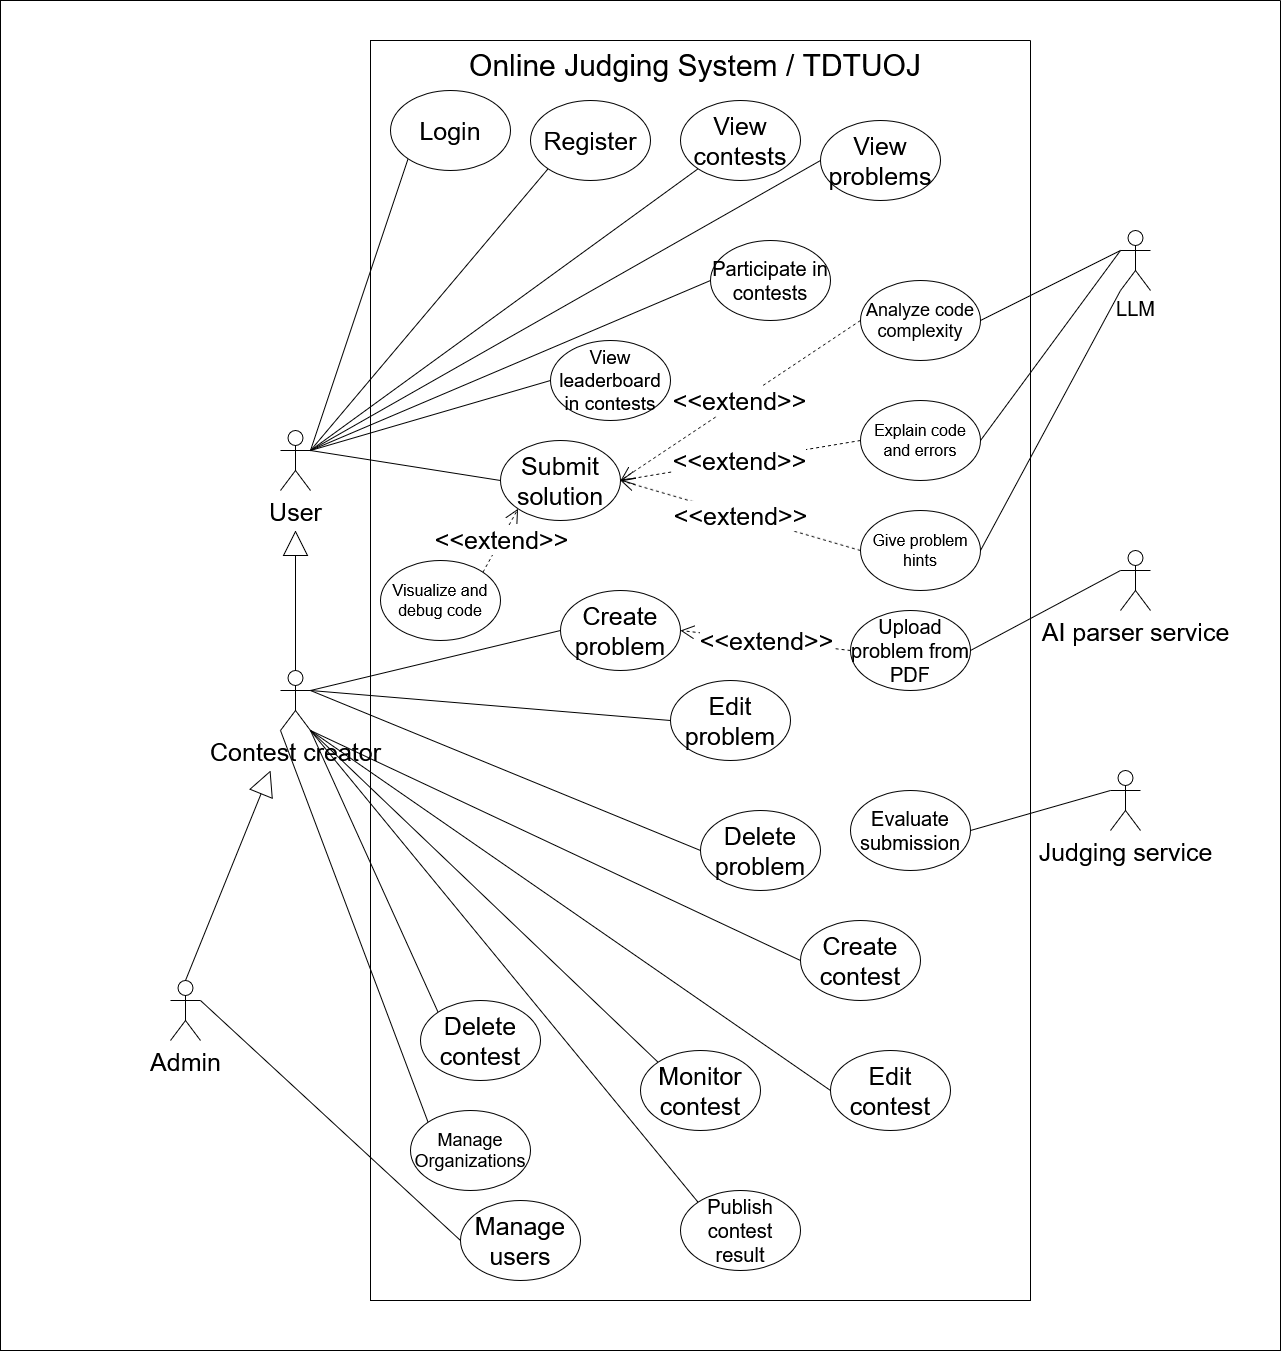
\includegraphics[width=0.92\textwidth]{figures/usecase.png}
  \caption{Sơ đồ Use Case tổng quan của hệ thống TDTUOJ}
  \label{fig:usecase}
\end{figure}

\section{Các tác nhân trong hệ thống}

\subsection{User (Người dùng)}

User là sinh viên hoặc người tham gia sử dụng hệ thống để luyện tập và tham gia cuộc thi. Đây là vai trò cơ bản nhất và là nền tảng của quan hệ kế thừa -- Contest Creator và Admin đều kế thừa toàn bộ quyền hạn của vai trò này. Theo sơ đồ Use Case, User có thể đăng nhập, đăng ký tài khoản, xem danh sách cuộc thi, xem danh sách bài toán, tham gia cuộc thi và xem bảng xếp hạng. Ngoài ra, User có thể nộp bài giải bằng C, C++, Java hoặc Python thông qua chức năng Submit solution, từ đó kích hoạt ba tính năng mở rộng: phân tích độ phức tạp code, giải thích code và lỗi, và gợi ý hướng giải -- tất cả được cung cấp bởi tác nhân ngoài \ac{LLM}. Chức năng Visualize and debug code cũng được liên kết với Submit solution như một tính năng hỗ trợ bổ sung.

\subsection{Contest Creator (Người tạo cuộc thi)}

Contest Creator là giảng viên hoặc người được cấp quyền tổ chức cuộc thi và quản lý bài toán. Ngoài toàn bộ quyền hạn của User, Contest Creator có thể tạo bài toán mới kèm bộ test cases, chỉnh sửa và xóa bài toán đã có. Chức năng Create problem có thể mở rộng bằng tính năng Upload problem from PDF -- thực hiện qua AI Parser Service, tự động chuyển đổi đề bài từ file \ac{PDF} thành dữ liệu có cấu trúc. Về tổ chức thi, Contest Creator có quyền tạo, chỉnh sửa, xóa, giám sát và công bố kết quả cuộc thi. Việc chấm bài được xử lý hoàn toàn tự động bởi Judging Service (Judge0).

\subsection{Admin (Quản trị viên)}

Admin là vai trò có quyền quản trị cao nhất trong hệ thống, kế thừa toàn bộ quyền hạn của Contest Creator. Ngoài ra, Admin có thêm hai chức năng quản trị toàn hệ thống: Manage users -- xem danh sách, chỉnh sửa thông tin, kích hoạt và vô hiệu hóa tài khoản -- và Manage Organizations, cho phép tạo và quản lý các tổ chức đại diện cho từng khoa hoặc lớp học.

\subsection{Các hệ thống bên ngoài}

TDTUOJ tích hợp với ba dịch vụ bên ngoài chuyên biệt. \ac{LLM} cung cấp ba tính năng hỗ trợ học tập được kích hoạt sau khi người dùng nộp bài: phân tích độ phức tạp code, giải thích code và lỗi, và gợi ý hướng giải. AI Parser Service trích xuất và chuyển đổi nội dung đề bài từ file \ac{PDF} thành dữ liệu có cấu trúc khi Contest Creator tạo bài toán mới. Judging Service thực thi và chấm điểm bài nộp thông qua Judge0, trả về verdict tương ứng.

\section{Thiết kế cơ sở dữ liệu}

\subsection{Sơ đồ thực thể -- quan hệ}

Sơ đồ \ac{ERD} trong Hình~\ref{fig:erd} thể hiện toàn bộ cấu trúc cơ sở dữ liệu của TDTUOJ với 20 bảng được tổ chức thành bốn nhóm chức năng: quản lý người dùng, quản lý bài toán, quản lý cuộc thi và quản lý bài nộp. Thiết kế đảm bảo tính toàn vẹn dữ liệu thông qua các ràng buộc khóa ngoại (\ac{FK}) và hỗ trợ hiệu quả các truy vấn phức tạp trong quá trình vận hành.

\begin{figure}[H]
  \centering
  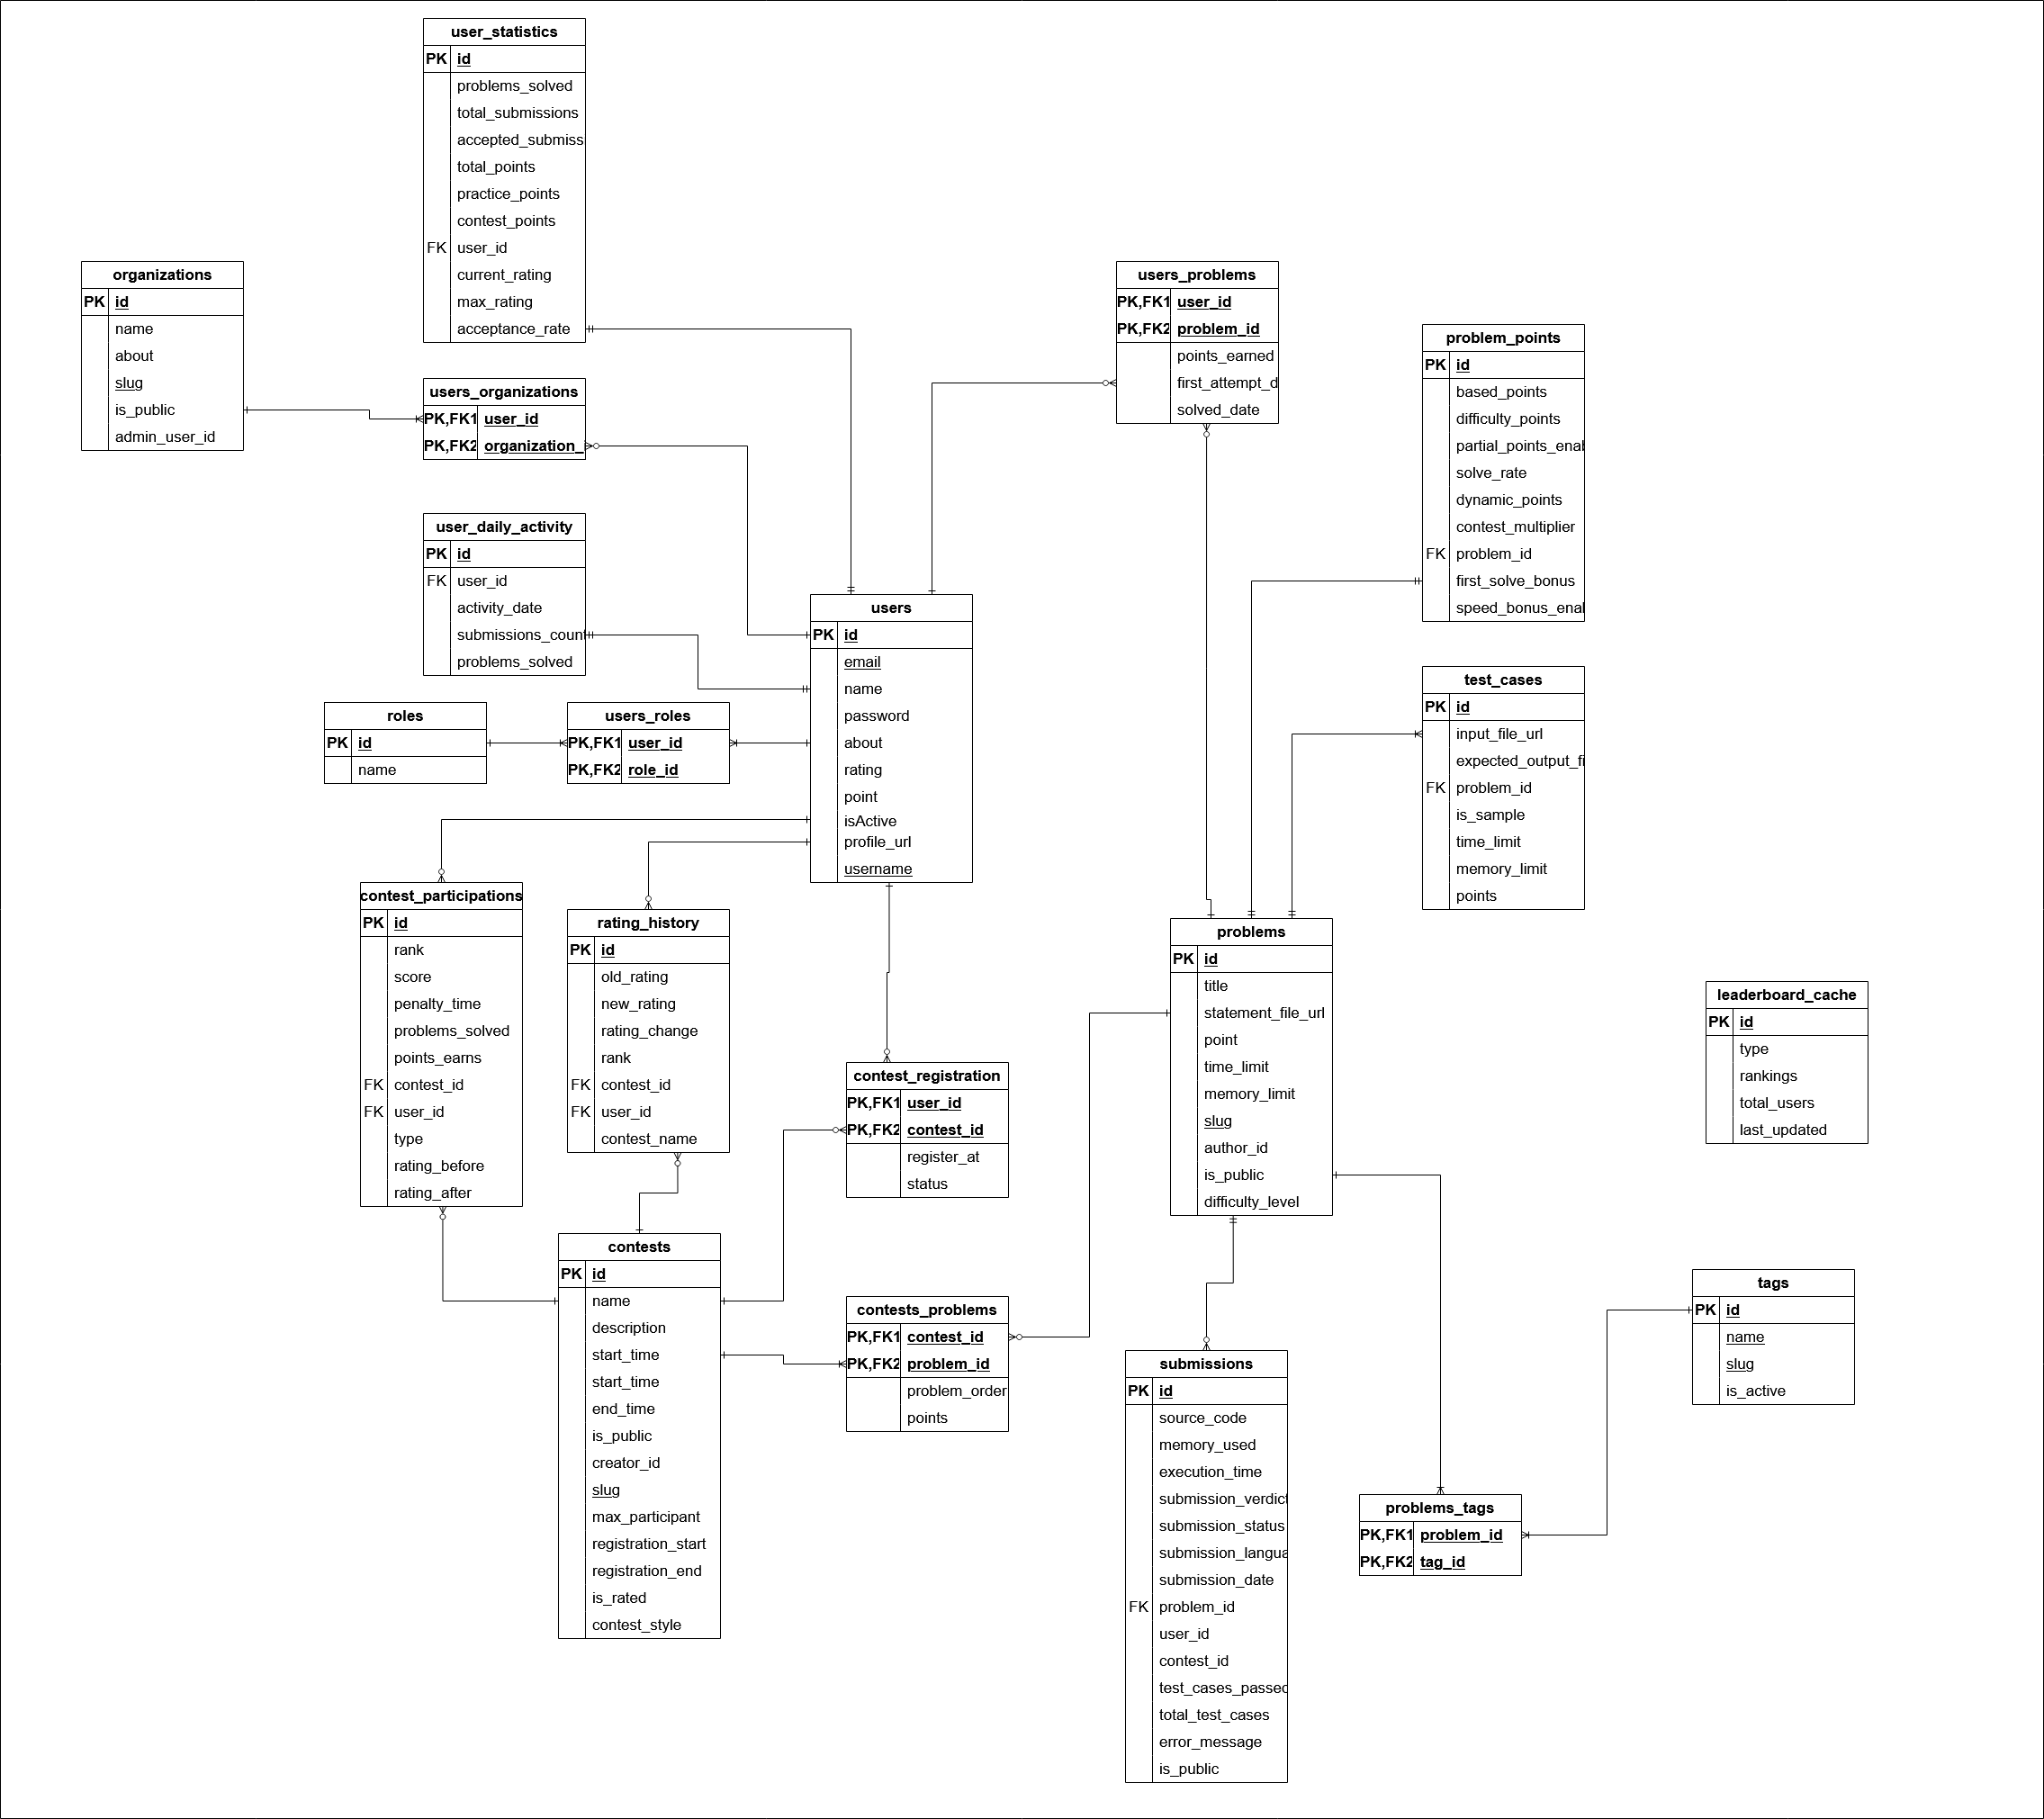
\includegraphics[width=\textwidth]{figures/erd.png}
  \caption{Sơ đồ thực thể -- quan hệ của hệ thống TDTUOJ}
  \label{fig:erd}
\end{figure}

\subsection{Nhóm bảng quản lý người dùng}

Nhóm bảng này xử lý toàn bộ dữ liệu liên quan đến tài khoản và hoạt động người dùng trong hệ thống.

Bảng \texttt{users} là bảng trung tâm của toàn hệ thống, lưu thông tin cơ bản của mỗi tài khoản gồm \texttt{email}, \texttt{name}, \texttt{password}, \texttt{username}, \texttt{rating}, \texttt{point}, \texttt{isActive} và \texttt{profile\_url}. Các trường \texttt{rating} và \texttt{point} phản ánh năng lực và thành tích tích lũy qua quá trình tham gia cuộc thi và luyện tập.

Bảng \texttt{roles} và bảng liên kết \texttt{users\_roles} hiện thực cơ chế phân quyền nhiều vai trò. Một người dùng có thể giữ nhiều vai trò đồng thời, mỗi vai trò được định nghĩa bằng trường \texttt{name}. Quan hệ nhiều-nhiều này được quản lý qua \texttt{users\_roles} với hai khóa ngoại \texttt{user\_id} và \texttt{role\_id}.

Bảng \texttt{organizations} lưu thông tin các tổ chức trong hệ thống với các trường \texttt{name}, \texttt{about}, \texttt{slug}, \texttt{is\_public} và \texttt{admin\_user\_id}. Quan hệ nhiều-nhiều giữa người dùng và tổ chức được quản lý qua bảng liên kết \texttt{users\_organizations}.

Bảng \texttt{user\_statistics} theo dõi các chỉ số tổng hợp của mỗi người dùng, bao gồm \texttt{problems\_solved}, \texttt{total\_submissions}, \texttt{accepted\_submissions}, \texttt{total\_points}, \texttt{practice\_points}, \texttt{contest\_points}, \texttt{current\_rating}, \texttt{max\_rating} và \texttt{acceptance\_rate}. Bảng này phục vụ chủ yếu cho các màn hình thống kê và bảng xếp hạng.

Bảng \texttt{user\_daily\_activity} ghi nhận hoạt động hàng ngày của người dùng qua các trường \texttt{activity\_date}, \texttt{submissions\_count} và \texttt{problems\_solved}, phục vụ hiển thị biểu đồ hoạt động theo ngày tương tự GitHub contribution graph.

Bảng \texttt{rating\_history} lưu lịch sử thay đổi rating qua từng cuộc thi, bao gồm \texttt{old\_rating}, \texttt{new\_rating}, \texttt{rating\_change}, \texttt{rank}, \texttt{contest\_id}, \texttt{user\_id} và \texttt{contest\_name}, giúp người dùng theo dõi sự tiến bộ theo thời gian.

\subsection{Nhóm bảng quản lý bài toán}

Nhóm bảng này quản lý nội dung bài toán, test cases, cấu trúc tính điểm và phân loại theo nhãn.

Bảng \texttt{problems} lưu thông tin chính của mỗi bài toán với các trường \texttt{title}, \texttt{statement\_file\_url}, \texttt{point}, \texttt{time\_limit}, \texttt{memory\_limit}, \texttt{slug}, \texttt{author\_id}, \texttt{is\_public} và \texttt{difficulty\_level}. Nội dung đề bài được lưu dạng file trên S3 bucket của AWS và trỏ đến qua \texttt{statement\_file\_url}, trong khi \texttt{slug} được dùng để tạo URL thân thiện cho từng bài toán.

Bảng \texttt{test\_cases} lưu các bộ dữ liệu kiểm thử gồm \texttt{input\_file\_url}, \texttt{expected\_output\_file\_url}, \texttt{is\_sample}, \texttt{time\_limit}, \texttt{memory\_limit} và \texttt{points}. Trường \texttt{is\_sample} phân biệt test case mẫu hiển thị công khai với test case ẩn chỉ dùng để chấm bài. Các trường \texttt{input\_file\_url} và \texttt{expected\_output\_file\_url} lưu đường dẫn tới file chứa dữ liệu test case, được lưu trữ trên dịch vụ S3 bucket của AWS.

Bảng \texttt{problem\_points} định nghĩa cấu trúc tính điểm với các trường \texttt{based\_points}, \texttt{difficulty\_points}, \texttt{solve\_rate}, \texttt{dynamic\_points}, \texttt{contest\_multiplier}, \texttt{first\_solve\_bonus} và \texttt{speed\_bonus}, cho phép tính điểm linh hoạt theo nhiều tiêu chí.

Bảng \texttt{tags} lưu danh sách nhãn phân loại bài toán theo chủ đề thuật toán với các trường \texttt{name}, \texttt{slug} và \texttt{is\_active}. Bảng liên kết \texttt{problems\_tags} quản lý quan hệ nhiều-nhiều giữa bài toán và nhãn qua hai khóa ngoại \texttt{problem\_id} và \texttt{tag\_id}.

Bảng \texttt{users\_problems} theo dõi lịch sử giải bài của từng người dùng với các trường \texttt{points\_earned}, \texttt{first\_attempt\_date} và \texttt{solved\_date}, cung cấp dữ liệu để tính thống kê và hiển thị trạng thái đã giải hay chưa cho từng bài toán.

\subsection{Nhóm bảng quản lý cuộc thi}

Nhóm bảng này xử lý toàn bộ vòng đời của một cuộc thi, từ khi tạo đến khi kết thúc và công bố kết quả.

Bảng \texttt{contests} lưu cấu hình cuộc thi với các trường \texttt{name}, \texttt{description}, \texttt{start\_time}, \texttt{end\_time}, \texttt{is\_public}, \texttt{creator\_id}, \texttt{slug}, \texttt{max\_participant}, \texttt{registration\_start}, \texttt{registration\_end}, \texttt{is\_rated} và \texttt{contest\_style}. Trường \texttt{contest\_style} cho phép cấu hình các kiểu thi khác nhau như ICPC hay IOI, ảnh hưởng trực tiếp đến cách tính điểm và xếp hạng.

Bảng liên kết \texttt{contests\_problems} quản lý danh sách bài toán trong một cuộc thi với các trường \texttt{contest\_id}, \texttt{problem\_id}, \texttt{problem\_order} và \texttt{points}, cho phép mỗi bài toán có trọng số điểm riêng trong từng cuộc thi.

Bảng \texttt{contest\_registration} ghi nhận thông tin đăng ký tham gia cuộc thi của người dùng với các trường \texttt{user\_id}, \texttt{contest\_id}, \texttt{register\_at} và \texttt{status}, phân biệt các trạng thái: đã đăng ký, đang chờ duyệt, hoặc bị từ chối.

Bảng \texttt{contest\_participations} theo dõi kết quả của từng thí sinh trong cuộc thi với các trường \texttt{rank}, \texttt{score}, \texttt{penalty\_time}, \texttt{problems\_solved}, \texttt{points\_earns}, \texttt{contest\_id}, \texttt{user\_id}, \texttt{type}, \texttt{rating\_before} và \texttt{rating\_after}. Đây là bảng chính phục vụ bảng xếp hạng và tính toán thay đổi rating sau mỗi kỳ thi.

Bảng \texttt{leaderboard\_cache} lưu dữ liệu bảng xếp hạng đã được tính toán sẵn với các trường \texttt{type}, \texttt{rankings}, \texttt{total\_users} và \texttt{last\_updated}, giúp tăng tốc độ truy vấn và giảm tải cho cơ sở dữ liệu khi nhiều người dùng xem bảng xếp hạng đồng thời.

\subsection{Nhóm bảng quản lý bài nộp}

Bảng \texttt{submissions} là trung tâm của luồng chấm bài, lưu toàn bộ thông tin về mỗi lần nộp. Các trường dữ liệu bao gồm \texttt{source\_code}, \texttt{memory\_used}, \texttt{execution\_time}, \texttt{submission\_verdict}, \texttt{submission\_status}, \texttt{submission\_language}, \texttt{submission\_date}, \texttt{problem\_id}, \texttt{user\_id}, \texttt{contest\_id}, \texttt{test\_cases\_passed}, \texttt{total\_test\_cases}, \texttt{error\_message} và \texttt{is\_public}. Trường \texttt{submission\_verdict} lưu kết quả cuối cùng (\ac{AC}, \ac{WA}, \ac{TLE}, \ac{MLE}, \ac{RE} hoặc \ac{CE}), còn \texttt{test\_cases\_passed} cung cấp thông tin chi tiết về số test case đã vượt qua, giúp người dùng định vị lỗi trong giải pháp của mình.

% ============================================================
% CHƯƠNG 4 – KẾT QUẢ ĐÃ THỰC HIỆN
% ============================================================
\chapter{Kết quả đã thực hiện}

Tính đến thời điểm báo cáo giữa kỳ, dự án đã hoàn thành một khối lượng đáng kể công việc thực tế trên cả hai phần backend và frontend.

\section{Backend -- Java Spring Boot}

Phần backend được triển khai bằng Java với Spring Boot. Kiến trúc tuân theo mô hình \ac{MVC} kết hợp \ac{REST}ful \ac{API}, trong đó mỗi tài nguyên được ánh xạ thành một endpoint \ac{HTTP} tương ứng với các phương thức GET, POST, PUT và DELETE.

\subsection{Quản lý người dùng}

Module quản lý người dùng là một trong những thành phần đầu tiên được hoàn thiện. Hệ thống hiện thực đầy đủ các chức năng xem danh sách người dùng, xem chi tiết từng tài khoản, cập nhật thông tin và thay đổi trạng thái hoạt động thông qua cơ chế kích hoạt và vô hiệu hóa -- tương tác trực tiếp với các bảng \texttt{users}, \texttt{roles} và \texttt{users\_roles}. Tất cả thao tác được bảo vệ bởi \ac{JWT}, đảm bảo chỉ Admin mới có thể thực thi các thao tác quản trị tài khoản.

\subsection{Quản lý bài toán}

Module quản lý bài toán cung cấp đầy đủ \ac{API} phục vụ cả Contest Creator và User thông thường, tương tác với các bảng \texttt{problems}, \texttt{test\_cases}, \texttt{problem\_points} và \texttt{problems\_tags}. Phía quản trị, hệ thống hỗ trợ tạo mới, chỉnh sửa và xóa bài toán cùng các thông số cấu hình như giới hạn thời gian, giới hạn bộ nhớ, mức độ khó và bộ test cases. Phía người dùng, hệ thống hiện thực chức năng truy xuất chi tiết bài toán qua \texttt{slug}, tạo URL thân thiện và phù hợp với tiêu chuẩn \ac{REST}ful hiện đại.

\subsection{Trực quan hóa thuật toán}

Tính năng trực quan hóa thuật toán đang được hoàn thiện. Sau khi có một bài nộp, người dùng có thể dùng chức năng này để trực quan hóa các biến và khối lệnh trong thuật toán bằng cách chạy các phần tử này theo từng bước (step). Tuy vậy, chức năng này vẫn chưa hoàn thiện và cần được điều chỉnh để phù hợp với nhu cầu sử dụng của sinh viên Khoa Công nghệ Thông tin.

\subsection{Xử lý bài nộp}

Luồng xử lý bài nộp là tính năng trọng tâm và đã được tích hợp đầy đủ với Judge0. Khi người dùng nộp bài, backend tiếp nhận mã nguồn và ngôn ngữ lập trình, chuyển tiếp đến Judge0 qua \ac{API}. Judge0 biên dịch và thực thi mã trong môi trường sandbox cô lập với các giới hạn lấy từ bảng \texttt{test\_cases}, rồi trả về verdict tổng thể. Toàn bộ kết quả -- verdict, thời gian thực thi, bộ nhớ sử dụng và số test case đã vượt qua -- được lưu vào bảng \texttt{submissions} và trả về frontend. Luồng xử lý được thiết kế theo mô hình bất đồng bộ, đảm bảo server không bị chặn trong khi chờ Judge0 hoàn thành.

\section{Tính năng hỗ trợ học tập bằng LLM}

Một điểm nổi bật của TDTUOJ là tích hợp \ac{LLM} để cung cấp ba tính năng hỗ trợ học tập thông minh, tương ứng với ba use case mở rộng từ Submit solution trong sơ đồ Use Case. Các tính năng này đã được hiện thực ở cả phía backend và frontend.

\subsection{Phân tích độ phức tạp code}

Sau khi bài nộp nhận kết quả \ac{AC}, hệ thống có thể gửi mã nguồn đến \ac{LLM} để nhận về phân tích độ phức tạp thời gian và không gian của giải thuật. Tính năng này giúp sinh viên không chỉ biết bài đúng hay sai mà còn hiểu được hiệu suất thực sự của giải pháp, từ đó có hướng tối ưu nếu cần.

\subsection{Giải thích code và lỗi}

Người dùng có thể yêu cầu \ac{LLM} giải thích chi tiết đoạn mã đã viết hoặc phân tích nguyên nhân lỗi trong các lần nộp không đạt. Hệ thống gửi mã nguồn cùng thông tin bài toán và thông báo lỗi đến \ac{LLM}, nhận về phần giải thích bao gồm mô tả logic tổng thể, phân tích các phần quan trọng và các điểm có thể cải thiện.

\subsection{Gợi ý hướng giải quyết bài toán}

Khi gặp khó khăn, người dùng có thể yêu cầu gợi ý mà không cần tiết lộ đáp án hoàn chỉnh. Hệ thống gửi thông tin bài toán đến \ac{LLM} và nhận về gợi ý có cấu trúc -- hướng dẫn người dùng suy nghĩ đúng hướng thông qua các câu hỏi dẫn dắt hoặc gợi ý về thuật toán phù hợp, giúp sinh viên phát triển tư duy giải quyết vấn đề một cách chủ động.

\section{Frontend -- React}

Phần frontend được xây dựng bằng React. Giao diện được tổ chức thành các component có khả năng tái sử dụng cao, mỗi tính năng lớn được đóng gói thành một module riêng biệt.

\subsection{Giao diện xem bài toán}

Giao diện xem chi tiết bài toán đã được hoàn thiện với khả năng tải và hiển thị thông tin bài toán dựa trên slug truyền vào qua URL. Nội dung hiển thị bao gồm tên bài toán, mô tả, ràng buộc đầu vào đầu ra, giới hạn thời gian và bộ nhớ, mức độ khó, danh sách nhãn thuật toán và các ví dụ test case mẫu -- lấy từ các bảng \texttt{problems}, \texttt{test\_cases} và \texttt{problems\_tags} qua backend \ac{API}.

\subsection{Giao diện quản lý người dùng}

Giao diện quản lý người dùng dành cho Admin cung cấp đầy đủ các chức năng hiển thị danh sách tài khoản, xem chi tiết, chỉnh sửa thông tin và vô hiệu hóa tài khoản. Các thay đổi trên giao diện lập tức gọi \ac{API} backend tương ứng và cập nhật trạng thái hiển thị theo kết quả phản hồi.

\subsection{Tính năng nộp bài}

Người dùng có thể nhập mã nguồn trực tiếp vào trình soạn thảo trên giao diện web, chọn ngôn ngữ lập trình và gửi bài nộp. Frontend xử lý toàn bộ luồng từ thu thập dữ liệu, gửi yêu cầu đến backend, chờ kết quả từ Judge0 và hiển thị verdict cuối cùng cùng thông tin chi tiết về số test case đạt, thời gian thực thi và bộ nhớ sử dụng.

% ============================================================
% CHƯƠNG 5 – HƯỚNG PHÁT TRIỂN
% ============================================================
\chapter{Hướng phát triển}

\section{Các tính năng còn lại cần hoàn thiện}

Mặc dù phần lớn chức năng cốt lõi đã được hiện thực, vẫn còn một số tính năng quan trọng cần hoàn thiện để hệ thống đạt đủ năng lực vận hành thực tế. Bảng xếp hạng theo thời gian thực trong cuộc thi cần được phát triển để cập nhật liên tục thứ hạng người tham gia, sử dụng dữ liệu từ bảng \texttt{contest\_participations} và \texttt{leaderboard\_cache}. Tính năng phân tích độ phức tạp thuật toán qua AI Analyzer và nhập đề bài tự động từ \ac{PDF} qua AI Parser Service cũng là các hạng mục còn lại cần hoàn thiện trong giai đoạn tiếp theo.

\section{Kế hoạch hoàn thiện}

\subsection{Hoàn thiện chức năng cuộc thi và tổ chức}

Ưu tiên hàng đầu là hoàn thiện toàn bộ vòng đời quản lý cuộc thi trên giao diện frontend. Hiện tại các \ac{API} backend cho cuộc thi đã sẵn sàng, nhưng phần giao diện dành cho Contest Creator vẫn cần được phát triển để tạo mới, chỉnh sửa, giám sát tiến trình và công bố kết quả một cách trực quan. Tính năng quản lý tổ chức cũng sẽ được hoàn thiện, cho phép Admin tạo và quản lý các tổ chức qua bảng \texttt{organizations} và \texttt{users\_organizations}, tạo ra cấu trúc phân cấp phù hợp với mô hình vận hành của một trường đại học. Ngoài ra, nhóm sẽ nghiên cứu ứng dụng bộ nhớ cache Redis để thực hiện việc xếp hạng người thi contest theo thời gian thực bằng điểm và thời gian giải được bài toán của người thi.

\subsection{Trực quan hóa thuật toán}

Như đã đề cập ở trên, nhóm sẽ hoàn thiện tính năng trực quan hóa thuật toán, cho phép sinh viên quan sát từng bước thực thi của các thuật toán phổ biến như sắp xếp, tìm kiếm, duyệt đồ thị và quy hoạch động thông qua hoạt ảnh minh họa trực tiếp. Người dùng có thể chọn thuật toán, nhập dữ liệu đầu vào tùy ý và điều chỉnh các bước hiển thị để theo dõi quá trình thực thi từng bước chi tiết của một thuật toán. Đây là công cụ học tập đặc biệt hữu ích cho sinh viên đang tiếp cận các khái niệm thuật toán lần đầu.

\subsection{Tích hợp trình gỡ lỗi}

Hệ thống sẽ tích hợp một trình gỡ lỗi trực tuyến vào giao diện nộp bài, cho phép người dùng đặt breakpoint, theo dõi giá trị biến tại từng bước thực thi và quan sát trạng thái chương trình ngay trên trình duyệt. Tính năng này giúp sinh viên tự chẩn đoán lỗi logic một cách chủ động, đồng thời rèn luyện kỹ năng debugging -- một kỹ năng thiết yếu trong nghề phát triển phần mềm. Tính năng này tương ứng với use case Visualize and debug code trong sơ đồ Use Case.

\subsection{Tích hợp AI và hoàn thiện các dịch vụ}

Sau khi hoàn thiện các chức năng quản lý cốt lõi, hệ thống sẽ tích hợp đầy đủ AI Analyzer vào luồng xử lý bài nộp để tự động phân tích và trả về độ phức tạp thuật toán ngay sau khi bài được chấp nhận, cùng với AI Parser Service để hỗ trợ giảng viên chuyển đổi đề bài từ \ac{PDF} một cách tự động. Ngoài ra, nhóm sẽ nghiên cứu ứng dụng các hàng đợi như RabbitMQ để xử lý bất đồng bộ các tác vụ chấm bài của Judge0, nhằm giảm tải cho hệ thống và đảm bảo việc chấm bài diễn ra mượt mà và ổn định.

\subsection{Hoàn thiện và đồng nhất giao diện người dùng}

Hiện tại, giao diện người dùng đã có những phần cơ bản nhưng vẫn còn thiếu sự đồng nhất về thiết kế và trải nghiệm. Nhóm sẽ hoàn thiện toàn bộ giao diện, đảm bảo tính nhất quán về màu sắc, kiểu chữ, bố cục và tương tác trên tất cả các trang. Việc này không chỉ nâng cao thẩm mỹ mà còn cải thiện trải nghiệm người dùng, giúp sinh viên dễ dàng tiếp cận và sử dụng hệ thống một cách hiệu quả.

\subsection{Kiểm thử và triển khai}

Giai đoạn cuối tập trung vào kiểm thử toàn diện và triển khai hệ thống lên môi trường production.

Về kiểm thử, nhóm sẽ thực hiện unit test cho từng module backend để đảm bảo tính đúng đắn của từng thành phần riêng lẻ, sử dụng JUnit 5 kết hợp Mockito để kiểm thử các lớp Service độc lập với cơ sở dữ liệu thực. Song song đó, nhóm sẽ tiến hành integration test để xác minh luồng hoàn chỉnh từ Controller qua Service đến Repository, đảm bảo các thành phần phối hợp đúng với nhau. Cuối cùng, stress test sẽ được thực hiện để đánh giá khả năng chịu tải -- đặc biệt ở các điểm nghẽn tiềm năng như luồng nộp bài đồng thời và truy vấn bảng xếp hạng trong thời gian diễn ra cuộc thi -- sử dụng công cụ Apache JMeter hoặc k6 để mô phỏng hàng trăm người dùng hoạt động cùng lúc.

Về giám sát hệ thống, sau khi triển khai nhóm sẽ tích hợp bộ công cụ quan sát \textbf{Prometheus} và \textbf{Grafana} để theo dõi sức khỏe hệ thống theo thời gian thực. Prometheus sẽ chủ động scrape metrics từ bốn nguồn: Spring Boot backend thông qua endpoint \texttt{/actuator/prometheus} do thư viện Micrometer cung cấp, Redis thông qua \texttt{redis\_exporter}, PostgreSQL thông qua \texttt{postgres\_exporter}, và máy chủ vật lý thông qua \texttt{node\_exporter}. Các metrics quan trọng cần theo dõi bao gồm tốc độ xử lý bài nộp, thời gian phản hồi của từng \ac{API} endpoint, độ dài hàng đợi submission trong Redis, tỉ lệ cache hit của leaderboard, và mức sử dụng CPU/RAM trong các đợt thi cao điểm. Grafana kết nối với Prometheus làm data source và trực quan hóa toàn bộ các chỉ số trên thành dashboard tập trung, đồng thời cấu hình alert rules để tự động gửi cảnh báo qua email hoặc Slack khi các ngưỡng quan trọng bị vượt -- chẳng hạn khi hàng đợi Redis tích lũy quá nhiều bài nộp chưa xử lý hoặc khi latency trung bình của Judge0 tăng đột biến.

Sau khi hệ thống vượt qua các ngưỡng kiểm thử, toàn bộ hạ tầng sẽ được triển khai lên \textbf{AWS}, tận dụng các dịch vụ phù hợp cho từng thành phần: EC2 cho backend và Judge0 workers, RDS cho PostgreSQL, ElastiCache cho Redis, và S3 cho lưu trữ file đề bài và test cases.

% ============================================================
% CHƯƠNG 6 – KẾT LUẬN
% ============================================================
\chapter{Kết luận}

\section{Tổng kết}

Đề tài xây dựng Hệ thống Chấm bài Trực tuyến TDTUOJ là một dự án có ý nghĩa thiết thực và phù hợp với nhu cầu thực tiễn của Khoa Công nghệ Thông tin, Trường Đại học Tôn Đức Thắng. Tính đến thời điểm báo cáo giữa kỳ, dự án không chỉ dừng lại ở giai đoạn phân tích và thiết kế mà đã tiến vào triển khai thực tế với nhiều kết quả cụ thể và có thể kiểm chứng.

Về phân tích và thiết kế, hệ thống đã có sơ đồ Use Case đầy đủ với ba tác nhân người dùng có quan hệ kế thừa rõ ràng và ba tác nhân bên ngoài, cùng sơ đồ \ac{ERD} hoàn chỉnh gồm 20 bảng phân thành bốn nhóm chức năng. Về triển khai, toàn bộ các module quản lý người dùng, bài toán, cuộc thi và bài nộp đã được hiện thực thành các \ac{REST}ful \ac{API} đầy đủ chức năng với bảo mật \ac{JWT}, tích hợp Judge0 cho việc chấm bài. Phía frontend đã hoàn thiện giao diện xem bài toán theo slug, quản lý người dùng, tính năng nộp bài và ba tính năng hỗ trợ học tập thông minh bằng \ac{LLM}. Toàn bộ mã nguồn được quản lý trên GitHub với 26 commit thể hiện tiến trình phát triển liên tục.

\section{Ý nghĩa của đề tài}

TDTUOJ không chỉ là một công cụ hỗ trợ giảng dạy đơn thuần mà là một nền tảng tổng thể có khả năng tạo ra tác động tích cực và lâu dài cho cộng đồng học thuật của nhà trường. Với sinh viên, hệ thống tạo ra môi trường luyện tập lập trình chuyên nghiệp với phản hồi tức thì, phân tích thuật toán chuyên sâu và hỗ trợ học tập thông minh từ \ac{LLM}. Với giảng viên, hệ thống giải phóng nguồn lực khỏi các công việc lặp đi lặp lại và nâng cao hiệu quả tổ chức thi cử. Ở tầm nhìn rộng hơn, TDTUOJ góp phần xây dựng văn hóa lập trình thi đấu tại \ac{TDTU}, đồng thời thể hiện năng lực nghiên cứu và phát triển phần mềm thực tiễn của sinh viên Khoa \ac{CNTT}.

% ============================================================
% TÀI LIỆU THAM KHẢO
% ============================================================
\newpage
\nocite{*}
\printbibliography[
  title   = {TÀI LIỆU THAM KHẢO},
  heading = bibintoc,
]

\end{document}